\newpage

\section{\textcolor{Plum}{Ergebnisse nach Entfernung der Extrema aus Frage 2 und Frage 3}}
\label{Add:Pruemper:neuer_ttest:frage_2_und_3}

\textcolor{red}{TODO: auch die Ergebnisse je Reihenfolge einbeziehen}
-> rohe Daten ohne die Werte auflisten
--> welche Tabelle will ich? - die große mit allen oder nur die der beiden Fragen?
-> Grafik mit dem grünen Signifikanzniveau einbinden

\begin{table}[H]
    \centering
    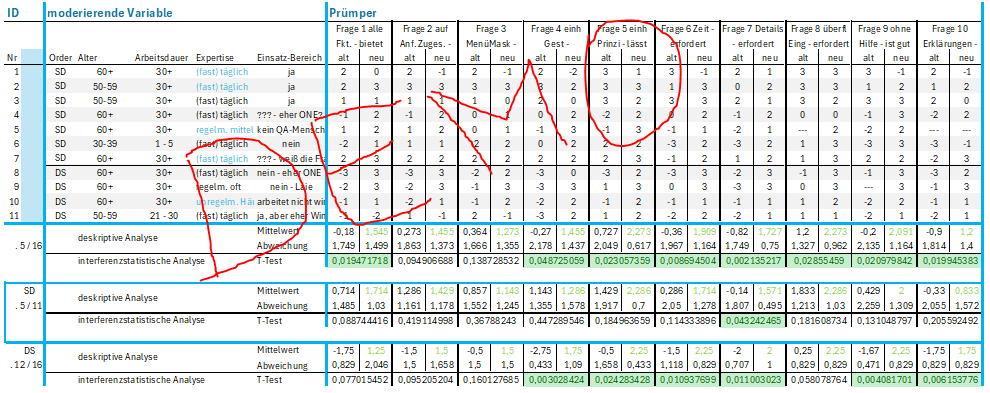
\includegraphics[width=0.65\textheight, angle=90]{Anhänge/Nutzerbefragung/prümper-Tabelle_demo.PNG}
    \caption{Nutzerbefragung nach Prümper der Fragen 2 und 3 nach Entfernung der Extrema - Tabellarische Daten \textcolor{red}{TODO: Bild austauschen}}
    \label{tab:Nutzerbefragung:rohe_Daten:ohne_Extrema_2_und_3}
\end{table}

\begin{figure}[H]
    \centering
    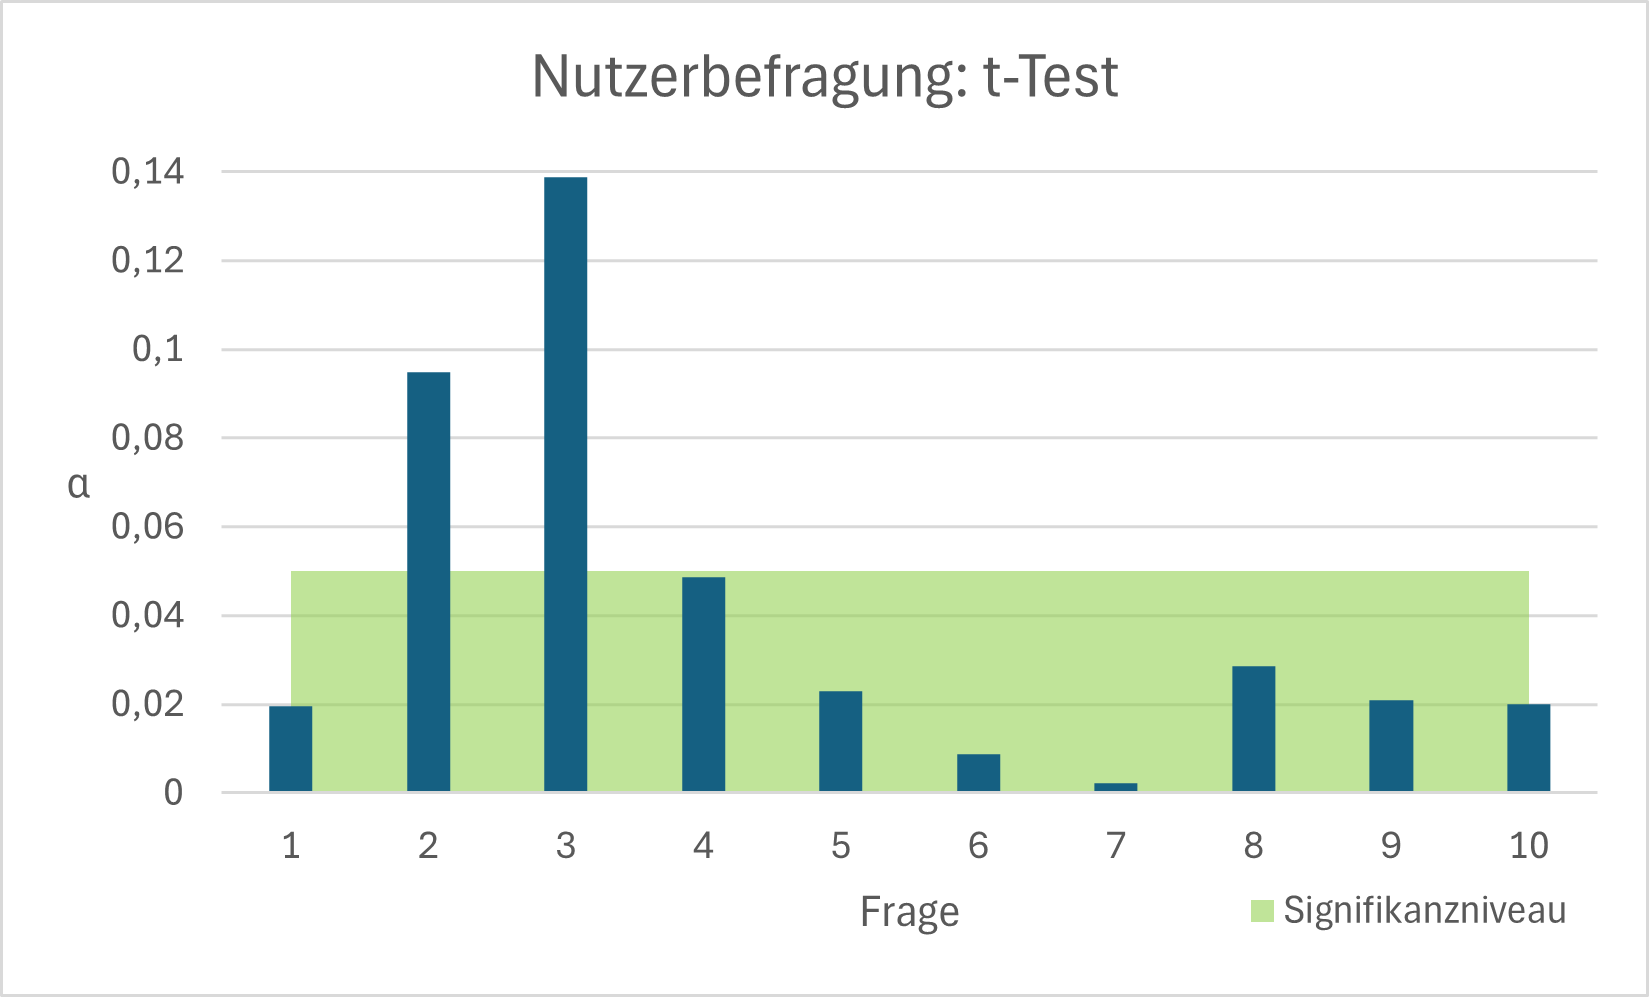
\includegraphics[width=0.8\linewidth]{Diagramme/pruemper_ttest.png}
    \caption{Nutzerbefragung - t-Test-Ergebnisse (Daten aus \autoref{tab:Nutzerbefragung:Differenz+ttest}) \textcolor{red}{TODO: neues Bild einfügen}}
    \label{fig:Nutzerbefragung:ttest+Signifikanzniveau:ohne_Extrema_2_und_3}
\end{figure}